
\documentclass[11pt, a4paper]{article}
%\usepackage{proj1}
\usepackage{natbib}
\usepackage{fancyhdr}  
\usepackage{subcaption}
\usepackage{caption}
\usepackage{graphicx}
\usepackage{numprint}
\usepackage{multirow}
\linespread{1.25} 
\setlength{\parindent}{0cm}
\graphicspath{{Images/}}
\usepackage{hyperref}
\usepackage{amsmath}
\usepackage{amsfonts}
\usepackage{amssymb}
\usepackage{amsthm}
\usepackage{mathtools}
\usepackage{commath}
\usepackage{bbm}

%\usepackage[sc,osf]{mathpazo}
\usepackage{subcaption}
\usepackage[a4paper, top=1in, left=1.0in, right=1.0in, bottom=1in, includehead, includefoot]{geometry} %Usually have top as 1in

\usepackage{listings}
\usepackage{color} %red, green, blue, yellow, cyan, magenta, black, white
\definecolor{mygreen}{RGB}{28,172,0} % color values Red, Green, Blue
\definecolor{mylilas}{RGB}{170,55,241}


\hypersetup{colorlinks,linkcolor={black},citecolor={blue},urlcolor={black}}
\usepackage{color}
\urlstyle{same}


\theoremstyle{definition}
\newtheorem{definition}{Definition}[section]

\newcommand{\adja}{q_a}
\newcommand{\adjb}{q_b}
\newcommand{\adjaB}{q_{a,\partial \Omega}}
\newcommand{\adjbB}{q_{b,\partial \Omega}}
\newcommand{\adjB}{q_{\partial \Omega}}
\newcommand{\Adja}{\mathbf{p}}
\newcommand{\Adjb}{q}
\newcommand{\adj}{q}
\newcommand{\Adjc}{{q}_{\partial \Omega}}
\newcommand{\ra}{\rho_a}
\newcommand{\rb}{\rho_b}
\newcommand{\w}{\mathbf{w}}
\newcommand{\x}{\mathbf{x}}
\newcommand{\f}{\mathbf{f}}
\newcommand{\ve}{\mathbf{v}}
\newcommand{\n}{\mathbf{n}}
\newcommand{\h}{\mathbf{h}}
\newcommand{\K}{\mathbf{K}}
\newcommand{\hr}{\widehat \rho}
\newcommand{\jf}{\mathbf j}

\DeclareMathOperator{\sgn}{sgn}
\DeclareMathOperator{\Grad}{Grad}
\DeclareMathOperator{\Div}{Div}
\DeclareMathOperator{\Lap}{Lap}
%	\begin{figure}[h]
%		\centering
%		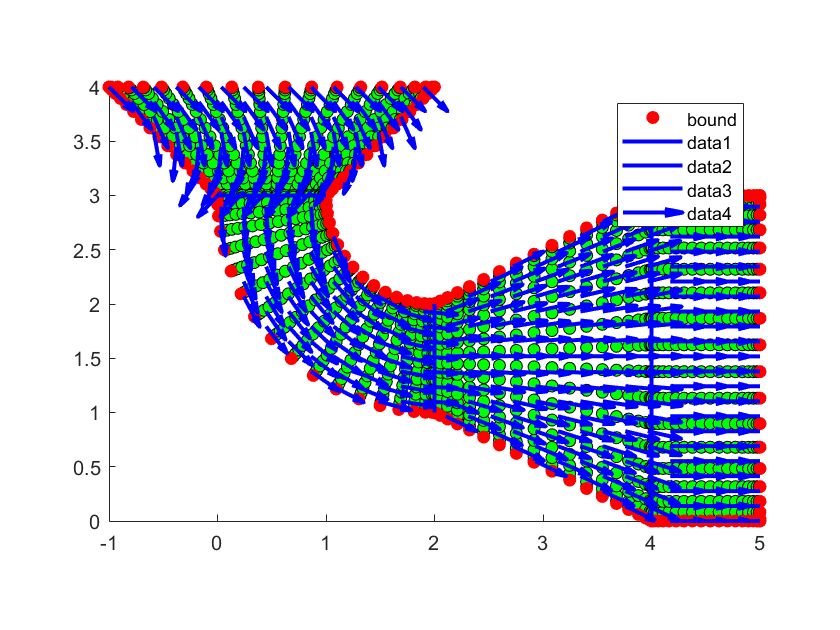
\includegraphics[scale=0.35]{F1.png}
%		\caption{Forward $\rho$ for $a = 0.01$} 
%		\label{F1}
%	\end{figure}

\begin{document}
We wrote the terms in * and ** into vector form as (*, **), but it should have been * + **. I think it has to be a sum, since the term we start out with in the cost functional is the scalar quantity
	\begin{align*}
		\frac{1}{2} \int_\Omega \nabla \times \w ^2 d\x &= \frac{1}{2} \int_\Omega \left(\frac{\partial w_2}{\partial x_1} - \frac{\partial w_1}{\partial x_2}\right)^2 d\x\\
		&= \int_\Omega \frac{1}{2} \frac{\partial w_2}{\partial x_1}\frac{\partial w_2}{\partial x_1} - \frac{\partial w_2}{\partial x_1}\frac{\partial w_1}{\partial x_2} + \frac{1}{2}\frac{\partial w_1}{\partial x_2}\frac{\partial w_2}{\partial x_1} d\x.
	\end{align*}
	We take the derivative with respect to $h_1$, $h_2$
	\begin{align*}
	 &\int_\Omega  \frac{\partial h_2}{\partial x_1}\frac{\partial w_2}{\partial x_1} - \frac{\partial h_2}{\partial x_1}\frac{\partial w_1}{\partial x_2} - \frac{\partial w_2}{\partial x_1}\frac{\partial h_1}{\partial x_2}+ \frac{\partial h_1}{\partial x_2}\frac{\partial w_1}{\partial x_2} d\x \\
	 =&\int_\Omega \frac{\partial h_2}{\partial x_1} \left(\frac{\partial w_2}{\partial x_1} - \frac{\partial w_1}{\partial x_2} \right) + \frac{\partial h_1}{\partial x_2}\left(\frac{\partial w_1}{\partial x_2} - \frac{\partial w_2}{\partial x_1} \right) d\x\\
	 =& \int_\Omega \frac{\partial}{\partial x_1}\left(h_2\frac{\partial w_2}{\partial x_1} - h_2\frac{\partial w_1}{\partial x_2} \right) - \left(h_2\frac{\partial^2 w_2}{\partial x_1^2} - h_2\frac{\partial^2 w_1}{\partial x_1 x_2} \right)\\
	 & + \frac{\partial}{\partial x_2}\left(h_1\frac{\partial w_1}{\partial x_2} - h_1\frac{\partial w_2}{\partial x_1} \right) - \left(h_1\frac{\partial^2 w_1}{\partial x_2^2} - h_1\frac{\partial^2 w_2}{\partial x_1 x_2} \right) d\x.
	\end{align*}
	Applying Green's theorem, we get
	\begin{align*}
		&\int_{\partial \Omega}\left(h_2\frac{\partial w_2}{\partial x_1} - h_2\frac{\partial w_1}{\partial x_2} \right) dx_1 + \left(h_1\frac{\partial w_1}{\partial x_2} - h_1\frac{\partial w_2}{\partial x_1} \right)dx_2\\
		&- \int_\Omega \left(h_2\frac{\partial^2 w_2}{\partial x_1^2} - h_2\frac{\partial^2 w_1}{\partial x_1 x_2} \right) + \left(h_1\frac{\partial^2 w_1}{\partial x_2^2} - h_1\frac{\partial^2 w_2}{\partial x_1 x_2} \right)  d\x.
	\end{align*}
	Rewriting the boundary terms we get
	\begin{align*}
		&\int_{\partial \Omega}\nabla \times \w h_2 dx_1 - \nabla \times \w h_1 dx_2\\
		&- \int_\Omega \left(h_2\frac{\partial^2 w_2}{\partial x_1^2} - h_2\frac{\partial^2 w_1}{\partial x_1 x_2} \right) + \left(h_1\frac{\partial^2 w_1}{\partial x_2^2} - h_1\frac{\partial^2 w_2}{\partial x_1 x_2} \right)  d\x.
	\end{align*}
	Green's Theorem can be written as
	\begin{align*}
		\int_{\partial \Omega} Ldx + M dy = \int_{\partial \Omega} \left(M, - L\right) \cdot \left(dy, - dx\right) = \int_{\partial \Omega} \left(M, - L\right) \cdot \n ds,
	\end{align*}
	where $ds = \sqrt{dx^2 + dy^2}$ and $\n$ chosen such that it is normalized and perpendicular to $(dx, dy)$.
	Therefore, we have
	\begin{align*}
		\int_{\partial \Omega}\nabla \times \w h_2 dx_1 - \nabla \times \w h_1 dx_2 &= \int_{\partial \Omega}\nabla \times \w \left(-h_1, - h_2\right)\cdot (dx_2, - dx_1) \\
		&= \int_{\partial \Omega}\nabla \times \w \left(-h_1, - h_2\right) \cdot \left(\frac{dx_2}{ds}, - \frac{dx_1}{ds}\right) ds,
	\end{align*}
	Consider the boundary term from my derivation	
	\begin{align}
		& \int_{\partial \Omega} \left(\nabla \times \w\right) \h_\bot \cdot \n d s\notag\\
		=&  \int_{\partial \Omega} \left(\nabla \times \w\right) \left(h_2, - h_1\right) \cdot (n_1, n_2) d s \label{eq1}.
	\end{align}
	These two formulations agree if $n_1 = \frac{dx_1}{ds}$ and $n_2 = \frac{dx_2}{ds}$. However, this doesn't quite make sense to me, since these are not normal to $dx_1$ and $dx_2$.

\end{document}